\chapter{Background}
\label{chap:background}

\section{Tandem Mass Spectrometry}
\label{sec:tandemMS}

\ac{MS} is a method for extracting the composition of a compound using its molecular weight \cite{broad_mass_spectrometry}. It measures the mass-to-charge ratio (m/z) of its ions to provide a spectral view of the compound. Due to its high precision and sensitivity, even the smallest molecules can be analyzed using Mass Spectrometry. Nowadays, Mass Spectrometers can analyze a sample within a few seconds with very high accuracy. This is the reason why it is the go-to method for analyzing unknown compounds \cite{scripps_mass_spectrometry}.

\subsection{Mass Spectrometry}

The basic MS process consists of 3 steps: ionization, mass analysis, detection \cite{broad_mass_spectrometry, garg2024mass}.
Firstly, the sample is ionized. This converts the molecules into charged ions and enables the manipulation by electric and magnetic fields. A common approach is electron ionization (EI). In this method, an electron beam is used to bombard the analyte molecule and knock an electron off, causing the molecule to split into charged ions and fragments according to their molecular structure \cite{scottElectronIonization}. This fragmentation is reproducible which makes the identification of a compound possible.
By using an electric or magnetic field, the ions are then separated based on their mass-to-charge ratio. One such method is using an ion trap, it uses an electric field to capture ions in a small space, holding them in stable orbits \cite{garg2024mass, chong2018clinical}. By gradually adjusting the field, ions are released sequentially by mass-to-charge ratio toward the detector. This allows for highly sensitive separation of the charged ions. The strength of the electric field when a specific ion is released from the tap determines its mass-to-charge ratio.
A detector will then quantify the separated ions \cite{garg2024mass}. These ions can be detected by using an electron multiplier. This device will amplify the signal strength of an incoming ion. When an ion strikes the electron multiplier's surface, it releases secondary electrons. These electrons are accelerated toward a series of dynodes (electrodes), each releasing more electrons upon impact. This cascade effect creates a large, amplified pulse of electrons from a single ion strike. The resulting electrical pulse is proportional to the number of ions, enabling the mass spectrometer to measure ion abundance (intensity) for each m/z value in the mass spectrum.

An example spectrum output from a mass spectrometer is shown as a histogram in Figure \ref{fig:mass_spectrum_example}.

\begin{figure}[h]
    \centering
    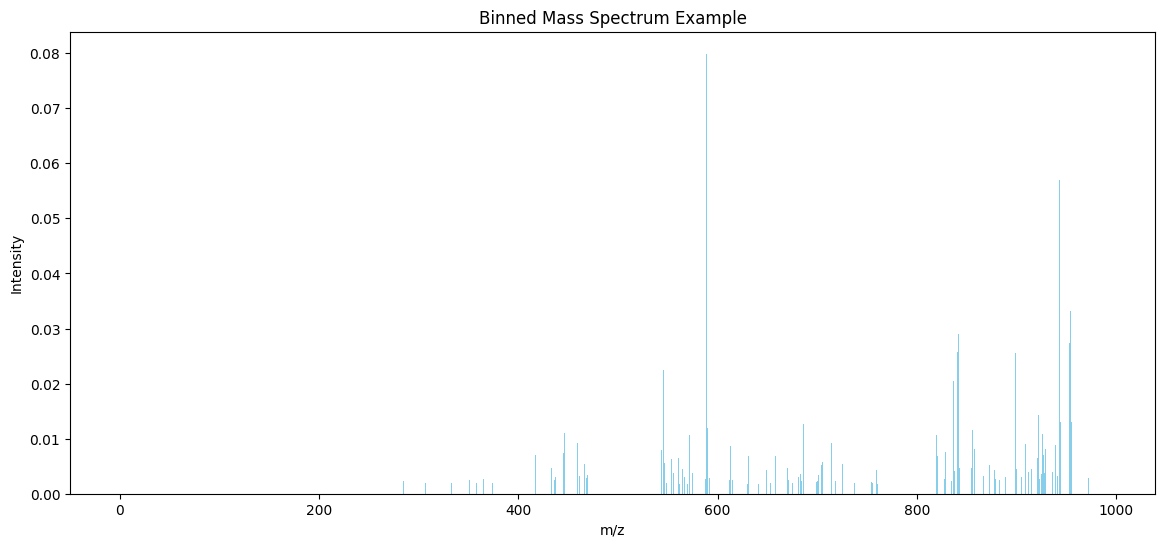
\includegraphics[width=\linewidth]{figures/background/mass_spectrum_example.png}
    \caption{A Mass Spectrum from GNPS, the peaks are binned using a histogram}
    \label{fig:mass_spectrum_example}
\end{figure}

\subsection{\acf{MS/MS}}

To determine the exact chemical structures of an input sample containing unknown molecules using mass spectrometry can be quite hard. Especially when the input sample contains a lot of different large molecules, the output from a single Mass Spectrometry analysis will describe an m/z spectrum of a mixture of ions. These different ions could have similar m/z values causing them to be inseparable. To distinguish them we can fragment ions with the same m/z range from the mixture using another round of Mass Spectrometry. This will fragment the ions further which allows them to be distinguished. This is in essence the goal of Tandem Mass Spectrometry (\acs{MS/MS} or MS$^2$). After ionization, it does multiple rounds of Mass Spectrometry (each with a separation step in between) before the detection step to increase the precision of the analysis \cite{antoniewicz2013tandem, nationalmaglabtand}. This way we can fragment and distinguish ions with similar m/z values.

In the separation step precursor ions are selected. These are ions that have overlapping m/z values that we want to fragment further. To achieve this, an isolation window is chosen with a certain m/z width \cite{defossez2023eight}. This window is used to slide over the spectrum generated by the first round of mass spectrometry to find these precursor ions. This selection is done either algorithmically or hard-coded. These precursor ions are then fragmented using collision-induced dissociation, ion-molecule reaction, or photodissociation. For example: Collision-induced dissociation uses the precusor ions in a gas stage to accelerate them towards neutral molecules \cite{wells2005collision}. The collision causes bonds within the ions to break, which fragments these precursor ions. These fragments can then be detected in the same way as the original mass spectrometry detector. Collision-induced dissociation can cause the molecular structure of an ion fragment to reform because a certain bond was broken, which will be detected as the wrong structure by the detector. Luckily this is mostly not the case \cite{molina2008comprehensive}.

The amount of fragmentation steps can be chosen arbitrarily, depending on known knowledge about the input molecules or precision needed for downstream analysis. Mass Spectrometry with a single fragmentation round is abbreviated as MS$^1$, tandem mass spectrometry with more than one round of fragmentation is often abbreviated as MS/MS or MS$^x$ with $x$ denoting the amount of fragmentation rounds.

\section{Molecular Representations}
\label{sec:molrepr}

This section discusses different molecular representations and their structures. Representations that are not frequently used in the molecular structure predicting domain are left out. Table \ref{tab:molecularreps} gives an overview of the molecular representations discussed in the following subsections.

%\begin{table}[h]
%    \centering
%	\setlength{\tabcolsep}{20pt}
%    \renewcommand{\arraystretch}{1.5}
%	\caption{
%		Different representations for the molecule Benzene. The Fingerprint representation shows only the first 40 bits for illustrational purposes, followed by three dots to indicate the truncation.
%	}
%	\begin{tabular}{ll}
%    		\toprule
%                    \textbf{Representation} & \textbf{Example} \\
%            \midrule
%    		      Chemical Formula & C$_6$H$_6$\\
%                    (Morgan) Fingerprint & 0000000000000000000000000000000000000010...\\
%                    InchI & InChI=1S/C6H6/c1-2-4-6-5-3-1/h1-6H\\
%                    InchIKey & UHOVQNZJYSORNB-UHFFFAOYSA-N\\
%                    SMILES & c1ccccc1\\
%                    DeepSMILES & cccccc6\\
%                    SELFIES & [C][=C][C][=C][C][=C][Ring1][=Branch1]\\
%    		\midrule
%    	\end{tabular}
%	\label{tab:molecularreps}
%\end{table}
\begin{table}[h]
    \centering
	\setlength{\tabcolsep}{20pt}
    \renewcommand{\arraystretch}{1.5}
	\caption{
		Different representations for the molecule Toluene (Methylbenzene). The Fingerprint representation shows only the first 40 bits for illustrational purposes, followed by three dots to indicate the truncation.
	}
    \resizebox{1.00\linewidth}{!}{
	\begin{tabular}{ll}
    		\toprule
                    \textbf{Representation} & \textbf{Example} \\
            \midrule
    		      Empirical Formula & C$_6$H$_5$CH$_3$\\
                    (Morgan) Fingerprint & 0000000000000000000000000000000000000000...\\
                    InchI & InChI=1S/C7H8/c1-7-5-3-2-4-6-7/h2-6H,1H3\\
                    InchIKey & YXFVVABEGXRONW-UHFFFAOYSA-N\\
                    SMILES & Cc1ccccc1\\
                    DeepSMILES & Ccccccc6\\
                    SELFIES & [C][C][=C][C][=C][C][=C][Ring1][=Branch1]\\
    		\midrule
    \end{tabular}
    }
	\label{tab:molecularreps}
\end{table}

\subsection{Empirical Formula}

The simplest and most well-known representation is the empirical formula. It is a textual representation that numbers the abundance of each element relative to each other. The empirical chemical formula does not describe any structural information and is therefore very unsuitable for describing specific molecular structures \cite{hartshorn2015brief}.

\subsection{Fingerprints}

To encode the chemical structure of a molecule, we could look at certain properties of the molecule instead of encoding the exact structure itself. This is in essence the purpose of molecular fingerprints. They represent properties of a molecule as a bitvector of a certain size which can be fixed or variable. Each bit then encodes the presence or absence of a certain property \cite{kuwahara2021analysis}. The properties that are encoded can vary. These are mostly human-curated specifically for a desired domain.

A few examples of different molecular fingerprints \cite{wigh2022review, kuwahara2021analysis, pharmacorefingerprints}:
\begin{description}
   \item[Structural / Topological fingerprints (e.g. MACCS Keys)]{Each bit represents the presence/absence of a certain molecular fragment. These are mostly used to measure molecular similarity.}
   \item[Circular/Radial fingerprints (e.g. Morgan Fingerprints (used in RDkit))]{These encode atom-centered neighborhoods iteratively. They capture local structural information but does not capture information on explicit connectivity.}
   \item[Pharmacophore fingerprints]{Encode chemical features such as structural properties related to binding.} 
   \item[Machine-learning-based / Embedding fingerprints]{Non-human curated bitvectors which are often a rounded output of an embedding layer from a neural network.}
\end{description}

These fingerprints provide a representation of a chemical structure that can explicitly store a lot of information about the properties of the molecule.
These bitvectors can be used very efficiently in well-established comparison algorithms which makes them very popular in certain machine learning applications that focus only on the properties that are encoded in the molecular fingerprint. Their main drawback is the way they are encoded. Because the molecular structure itself is not encoded as a whole, even with structural fingerprints it is very hard to extract the exact molecular structure because some structural information is lost \cite{kretschmer2023small}. Different chemical structures can also encode to the same bitvector, because they share the same properties, which can cause confusion. For these reasons, this molecular representation is not desired for describing a molecular structure \cite{dablander2024sort}.

\subsection{InChI}

The International Chemical Identifier (InChI) is a standardized textual representation of a molecular structure developed by IUPAC \cite{heller2015inchi}. InChI has a bijective relation with all molecular structures, which allows each structure to be uniquely represented to prevent ambiguity. It was originally developed (and is still mostly used) for search algorithms to distinguish between different representations of the same molecule. An InChI consists of layered information:
\begin{description}
    \item[Main Layer]Defines core molecular connectivity and hydrogen positions.
    \item[Charge Layer]Captures formal charge states.
    \item[FixedH layer]Allows to distinguish tautomers by their mobile H atoms.
    \item[Stereochemistry Layer]Encodes chiral centers and double-bond configurations.
    \item[Isotopic Layer]Represents isotopic variations.
    \item[Reconnected layer]Metal-containing compounds are split to prevent ambiguity, the original metal bonding scheme is stored here.
\end{description}

Each Identifier starts with "InchI=", followed by each layer seperated by a forward slash character. Not all layers have to be present to describe a valid InChI, redundant or non-relevant information can be omitted if the base relation of InchI still holds. This layered textual structure allows the format to be somewhat human-readable.

\subsubsection{InchIKey}

A main drawback of InchI is its length. For big molecular structures this can be very large.
Therefore, to further improve search methods, the InchI can be hashed to drastically reduce its size.
This is exactly what InchIKey achieves.
It is a 27-character compacted representation calculated by combining blocks of SHA256 hashes converted to base26.
These blocks are calculated by hashing the different layers from the InchI string.
The first block, consisting of 14 letters, encodes the core molecular constitution using the main layer.
The second block, with a length of 10 letters, is created by using 8 letters from the hashed remaining layers and 2 letters to denote the InchI type (S for standard N for non-standard) and version (A for version 1).
The last block containing one letter is used to describe in which protonation state the molecule is, with N being neutral.
These three blocks are separated by a hyphen character.

Because InchIKey is hashed, in theory it loses the bijective relation to the chemical structures, as hash collisions (2 InchI mapping to the same InchIKey) are possible.
\textcite{pletnev2012inchikey} have proven however that this probability is close to the theoretical expectation which is almost negligible.

While InchI's can be used to reconstruct an exact molecular structure, the one-way encoding using hashing prevents this with InchIKeys. They are only useful for database lookups as the InchIKey itself does not allow any structural information to be extracted. 

\subsection{SMILES}

A \ac{SMILES} string provides a linear textual representation of a molecular structure using ASCII characters.
It was developed to mimic the structure of natural language with its linear string of symbols, while also maximizing its simplicity \cite{weininger1988smiles}. The SMILES generation rules are kept relatively simple while still holding the desired requirements for a chemical notation language. It balances the human-readability with optimization for computer efficiency, striving to be human- and machine-friendly.

SMILES describe a molecular structure as a two-dimensional graph. It encodes the connectivity between atoms.
The SMILES generation rules are as follows:

\begin{itemize}
    \item Atoms are depicted by their atomic symbols in square brackets (except for some organic elements) with the second letter being lowercase. (e.g. [Fe])
    Attached hydrogens (the symbol H with an optional digit following) and formal charges (+ or - with an optional digit following) should also be denoted inside the square brackets.
    \item Bonds are represented by: - for single bonds, = for double bonds and \# for triple bonds. Single bond characters are usually ignored.
    \item Branches are depicted by encapsulation with parentheses.
    \item Cycles are split and represented in any order starting and ending with the same single digit denoting the start and end of the cycle.
    \item Disconnected structures are represented independently with a period used for separation.
    \item Aromatic ring structures are depicted by using lower case letters.
\end{itemize}

These generation rules are still flexible, which allows for multiple SMILES to be "synonyms" of each other.

Because SMILES only represent two-dimensional graphs and captures only the connectivity between atoms, 
they generally lack explicit three-dimensional information such as the precise spatial orientation, conformational flexibility, and subtle stereochemical details unless additional annotations are included. Without these extra annotations, multiple chemical structures could map to the same SMILES string, standardization is thus needed to distinguish similar molecular structures.\cite{heller2015inchi}.   

\subsubsection{DeepSMILES}

Because SMILES strives to mimic natural language, the recent breakthroughs in natural language processing using auto-regressive neural networks proved its utility for chemical structure generation. Its biggest drawback however is that the representation allows for syntactical errors by either unbalanced parentheses and unbalanced ring depictions \cite{o2018deepsmiles}. DeepSMILES \cite{o2018deepsmiles} addresses these issues. It is a chemical representation built on the same fundamentals as SMILES, with the exception of these two main issues. In DeepSMILES, ring structures only have a digit at the end to denote the ring size, which implicitly encodes the starting position. The unbalanced parentheses problem is solved by only using closing parentheses. The closing parentheses are then repeated, with the amount being equal to the branch length. With these changes DeepSMILES can be converted easily to SMILES without any loss of data.

These optimizations for SMILES strings make sure that even a string,
sampled with random (SMILES) characters (except for the opening bracket),
depicts a valid DeepSMILES string,
which is an important feature in autoregressive generation. However it does not address the problem that some strings may violate basic chemistry rules such as the maximum number of valence bonds between atoms \cite{krenn2020self}.

\subsection{SELFIES}

Another textual molecular representation that strives to have the same benefits as SMILES without the possible syntactical errors is \ac{SELFIES} \cite{krenn2020self}.
Unlike DeepSMILES, thay also address the chemical validity of strings. This is achieved by using a context free grammar~\cite{lo2023recent}. A SELFIES string is a combination of tokens. These tokens are restricted by a constraint function to be chemically viable.
This is the key aspect that allow SELFIES to be robust. There are four different kind of tokens:

\begin{description}
    \item[Atom Token] Following the notation of \textcite{lo2023recent}, an atom token has the form:
    \[[\beta\alpha_{iso}\alpha_{elem}\alpha_{chiral}\alpha_{H}\alpha_{\pm}]\]
    where:
    \begin{align*} 
    \beta &\in  \{\varepsilon, = , \#,/, \textbackslash\} \\ 
    \alpha_{iso} &\in  \{\varepsilon,1,2,3,...\} \\
    \alpha_{elem} &\in  \{element\ symbols\} \\ 
    \alpha_{chiral} &\in  \{\varepsilon, @, @@\} \\
    \alpha_{H} &\in  \{\varepsilon,H0,H1,...,H9\} \\
    \alpha_{\pm} &\in  \{\varepsilon,+1,-1,+2,-2,+3,...\}
    \end{align*}
    Beta describes a SMILES-like bond, the alphas describe isotope number, atomic number, chirality, number of attached hydrogens and charge respectively \cite{lo2023recent}. A lot of information is described with one token, whereas in SMILES there would be a lot of different symbols used.
    
    \item[Branch Token] Following the notation of \textcite{lo2023recent}, a branch token has the form:
    \[[\beta Branch\ \ell]\]
    where:
    \begin{align*} 
    \beta &\in  \{\varepsilon, = , \#\} \\ 
    \ell &\in \{1, 2, 3\}
    \end{align*}
    Again Beta is a SMILES-like bond. A branch token is only put at the end of a branch (similar to DeepSMILES) with the next $\ell$ tokens describing the length of the branch by using predefined tokens to represent certain values. When there are no next tokens, 0 is used.

    \item[Ring Token] Following the notation of \textcite{lo2023recent}, a ring token has one of 2 forms:
    \begin{align*} 
    &[\beta Ring\ \ell] \\ 
    &[\beta_1\beta_2 Ring\ \ell]
    \end{align*} where: \begin{align*} 
    \beta &\in  \{\varepsilon, = , \#\} \\
    \ell &\in \{1, 2, 3\} \\
    \beta_1,\beta_2 &\in \{-, /, \textbackslash\} \\
    \beta_1 = -& \Rightarrow \beta_2 \neq - \\
    \beta_2 = -& \Rightarrow \beta_1 \neq -
    \end{align*}
    Similar to branch tokens, ring tokens are put at the end of a ring enclosure. The size of the ring is calculated in the same way as the length of the branch for branch tokens.

    \item[Miscellaneous Tokens] Miscellaneous symbols are required for SMILES to be easily translatable to SELFIES. An example of a miscellaneous token is the dot symbol. Just as in SMILES it represents a disconnected structure.
    
\end{description}

Because these tokens encode so much information that is stored by multiple symbols in SMILES, by only using a combination of valid tokens, SELFIES strings are completely robust. This means that it always encodes a valid molecular structure while also being able to represent every possible molecule \cite{lo2023recent}. If we would randomly sample from a complete set of tokens, which can be constructed by exhausting the constraint function defined in SELFIES, the result would always map to a valid molecular structure. This is a key aspect which proves its usefulness in the autoregressive generation of SELFIES.

\section{Evaluation Metrics}
\label{sec:evalmetrics}

Quantifying the similarity of molecular representations is crucial for evaluating machine learning models that try to predict these representations. The similarity metric should describe how similar the actual molecular structures of two representations are. The most naive similarity metrics often only describe how similar the representations are to each other without taking the underlying chemical structure into account. This, however, will hinder generalization for the overall molecular structure prediction problem. More advanced metrics are required.

A distinction also needs to be made between structural similarity and property similarity. Property similarity is often the preferred metric in biological settings that are more interested in the properties of the molecules \cite{safizadeh2021improving}. Because this thesis is about predicting molecular structures, only structural similarity metrics are discussed.

\subsection{Tanimoto Similarity}
The molecular structure can't be directly derived from fingerprints because they don't store complex structural information \cite{kretschmer2023small}. This is a problem for calculating the similarity of the underlying molecular structure of two fingerprints, as we can't construct molecular graphs to calculate an exact structural similarity metric. We have to resort to similarity metrics on fingerprints themselves that would estimate the structural similarity.

Molecular fingerprints are bitvector representations. A naive way to compare two bitvectors would be to calculate the sum of the logical 'and' operation divided by the length of the bitvector, in essence counting the number of bits that are the same. This would only work if the value of each bit has no correlation with any other bit and each bit in the bitvector has an equal occurrence probability. This is not true for molecular fingerprints. They are known to be very sparse and have a non-uniform distribution. For example: Figure \ref{fig:bit_frequency_fingerprints} shows the activation frequency per bit position for a typical fingerprint. It is clear that these are not uniformly distributed with some bits having a very high activation frequency (above 70\%) and a few bits not even being active once. It is clear that the activation frequency of most bits is very low, causing the fingerprints to be sparse.

\begin{figure}[h]
    \centering
    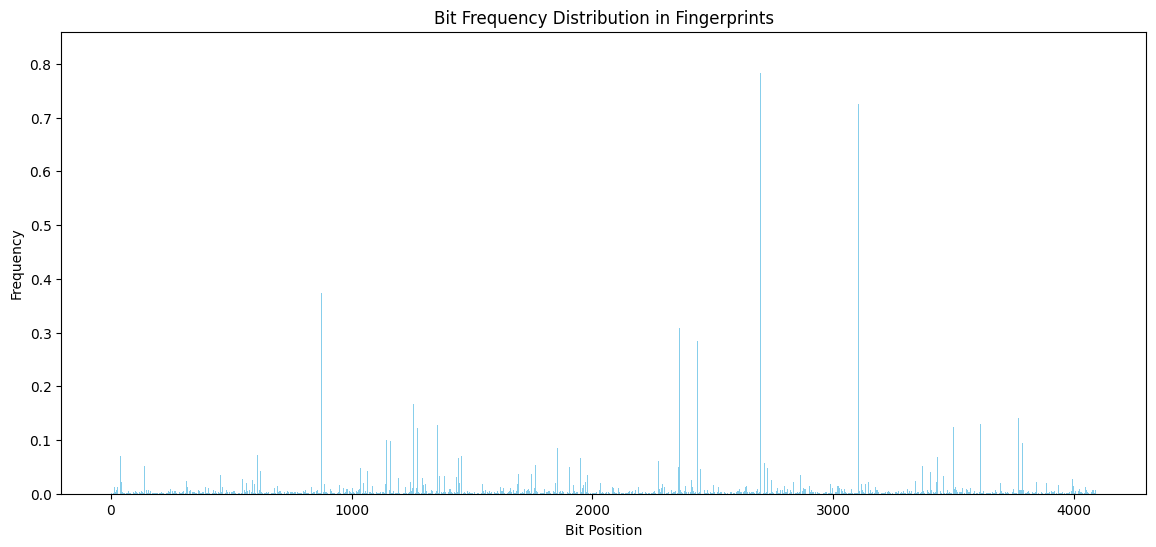
\includegraphics[width=\linewidth]{figures/background/bit-frequency-distribution-fingerprints.png}
    \caption{Bit frequency distribution of Morgan Fingerprints in GNPS dataset}
    \label{fig:bit_frequency_fingerprints}
\end{figure}

A similarity metric that takes the sparseness of these fingerprints into account is the Tanimoto similarity (i.e. Jaccard index). Using the notation by \textcite{mathieson2017computer}  the Tanimoto similarity of 2 real vectors A and B is defined as follows:
\[Tc_G(A,B) = \frac{\sum\limits^n_{i=1}{A_iB_i}}{\sum\limits^n_{i=1}{A_i^2} + \sum\limits^n_{i=1}{B_i^2} - \sum\limits^n_{i=1}{A_iB_i}}\]

For vectors containing only binary values this can be simplified as \cite{mathieson2017computer}:
\[Tc(A, B)=\frac{c}{a + b - c}\]
Where $A$ and $B$ are 2 bitvectors. $a$ and $b$ are the amount of activated bits for the 2 bitvectors respectively. The amount of bits that are activated in both $A$ and $B$ is represented with $c$. The Tanimoto similarity of two fingerprints is the ratio of shared properties to the total number of unique properties in the fingerprints \cite{mathieson2017computer}, or, in other words, the intersection over union of the 2 bit sets. Only properties that are present in one of the fingerprints are taken into account for the calculation. This makes the metric robust for sparse bitvectors.

By calculating the Tanimoto similarity of structural fingerprints (for which the properties represent the presence of unique substructures) or radial fingerprints (which has local structural properties) we can estimate the structural similarity of the underlying molecular structure.

\textcite{bajusz2015tanimoto} have benchmarked different metrics and shown that the Tanimoto similarity metric should be considered as one of the best similarity metrics on molecular fingerprints. It is still not an optimal molecular similarity metric for when the exact structures are known, as fingerprints are unable to store enough structural information. By converting the exact structure to a fingerprint there is a loss of information \cite{kretschmer2023small}.

\subsection{MCES Distance}
For molecular representation where we can accurately extract the molecular structure (InchI, SMILES, DeepSMILES, SELFIES), we can construct a molecular graph of the molecule \cite{wigh2022review}. Molecular graphs are labeled graphs where edges describe bonds and nodes describe atoms \cite{kretschmer2023small}. From two molecular graphs, a graphical similarity metric can then be calculated to get an accurate molecular similarity metric. 

One such graphical metric that extrapolates well to chemical structure similarity is the \ac{MCES} distance \cite{kretschmer2023small}. The MCES distance of two graphs A and B is defined as follows:
\[d_{MCES} = E_A + E_B - 2E_{MCES_{AB}}\]
Where $E_A$ is the amount of edges in graph A, and $MCES_{AB}$ is the maximum common edge subgraph of A and B, this is the largest graph for which all edges (with their corresponding end nodes) are present in A and B. Intuitively the MCES distance is the minimal amount of edges we have to remove from both graphs to get isomorphic graphs \cite{kretschmer2023small}. Or from a chemistry standpoint, by \textcite{kretschmer2023small} "the 'number of chemical reactions' required to transform one molecule into another".

Even with the optimizations proposed by \textcite{kretschmer2023small}
(e.g. They use a maximum distance upper bound.
Exact MCES distances are only calculated when they are estimated to be lower than this bound,
otherwise the upper bound is returned, termed the myopic MCES distance),
the calculation of the MCES is NP-hard and thus very compute-intensive.
When the MCES distance is used for evaluation in a machine learning molecular structure prediction setting,
this will slow down evaluation time drastically compared to a faster evaluation metric, e.g. Tanimoto similarity on fingerprints.

\section{Identifying molecules from \ac{MS/MS}}
\label{sec:relatedwork}

There have been a lot of studies on the use of Mass Spectrometry data to predict chemical structures. Table \ref{tab:relworkpapers} lists the most credited papers with their models, showing the evolution of the field of molecular structure prediction using MS/MS data.
"De novo" in this context means that a chemical structure is predicted directly without the use of candidate selection. Candidate selection models rank the chemical structures in a database by how closely they relate to the input structure. "De novo" models are able to predict a chemical representation without a reference dataset. The chemical structure can be derived by these models by only using the features learned from the training set.

\begin{table}[h]
	\setlength{\tabcolsep}{3pt}
        \renewcommand{\arraystretch}{1.5}
	\caption{
		Models predicting molecular structures from most cited papers
	}
	\resizebox{1.00\linewidth}{!}{
	\begin{tabular}{p{4cm}p{3cm}p{3cm}p{3cm}p{1cm}p{1.5cm}}
		\toprule
                \textbf{Model/Paper} & \textbf{Input Data} & \textbf{Model Output} & \textbf{Architecture} & \textbf{De Novo} & \textbf{Year Published} \\
            \midrule
		      %https://pubmed.ncbi.nlm.nih.gov/22815355/
                 FingerID \cite{heinonen2012metabolite}  & MS/MS & Fingerprints & SVMs & No & 2012 \\
                 %https://www.pnas.org/doi/10.1073/pnas.1509788112
                 CSI:FingerID \cite{duhrkop2015searching}  & MS/MS & Fingerprints & Fragmentation trees + SVMs & No & 2015 \\
                 %https://www.nature.com/articles/s41592-019-0344-8
                 Sirius 4 \cite{duhrkop2019sirius}  & MS/MS & Fingerprints & Fragmentation trees + SVMs & No & 2019 \\
                 %https://link.springer.com/article/10.1007/s11306-020-01726-7
                 MetFID \cite{fan2020metfid} & MS/MS & Fingerprints & MLP & No & 2020 \\
                 %https://www.biorxiv.org/content/10.1101/2022.12.30.522318v1
                 MIST \cite{goldman2023annotating}   & MS/MS & Fingerprints & Transformer & No & 2022 \\
                 %https://chemrxiv.org/engage/chemrxiv/article-details/6626775021291e5d1d61967f
                 DreaMS \cite{bushuiev2024emergence}  & MS/MS & Embedding Vector & Transformer & No & 2023 \\
                
                 \midrule
                 %https://pubs.acs.org/doi/10.1021/acscentsci.7b00572
                 \textcite{gomez2018automatic} & SMILES  & (latent space +) SMILES    & VAE + RNN & Yes & 2018 \\
                 %https://chemrxiv.org/engage/chemrxiv/article-details/613e83a7656369203b2a249b
                 Spec2Mol \cite{litsa2021spec2mol} & MS/MS & SMILES & CNN + GRU & Yes & 2021 \\
                 %https://www.nature.com/articles/s41592-022-01486-3
                 MSNovelist \cite{stravs2022msnovelist} & Fingerprints  & SMILES    & RNN     & Yes     & 2022 \\
                 %https://www.mdpi.com/2218-273X/11/12/1793
                 MassGenie \cite{shrivastava2021massgenie} & in silico MS/MS & SMILES & Transformer & Yes & 2021 \\
                 %https://doi.org/10.26434/chemrxiv-2023-vsmpx-v4
                 MS2Mol \cite{butler2023ms2mol} & MS/MS & SMILES & Transformer & Yes & 2023 \\
		\midrule
	\end{tabular}
	}
	\label{tab:relworkpapers}
\end{table}

% Extra sources
%https://jcheminf.biomedcentral.com/articles/10.1186/s13321-016-0116-8

\subsection{Fingerprint prediction}

One of the first models to only use tandem mass spectrometry to predict chemical features in the form of a fingerprint is \textbf{FingerID} \cite{heinonen2012metabolite}. It is a relatively simple model that first converts the peaks of the tandem mass spectrometry output to discrete binned values. These are then passed to a set of kernels in a \ac{SVM} learning model to predict structural molecular fingerprints. These fingerprints could then be used to extract certain properties of the molecule or be used as a search key to compare against a database of known molecular structures with their fingerprints (e.g. PubMed), to rank the most similar structures. 

\textbf{CSI:FingerID} \cite{duhrkop2015searching} significantly improves the methods proposed in FingerID by first computing fragmentation trees from the mass spectrometry spectra to better explain the fragmentation spectrum.
Fragmentation trees describe the fragmenting process a precursor ion underwent during mass spectrometry \cite{bocker2008towards}. The tree-like structure uses fragments as nodes and edges to stipulate that a child node is the result of the fragmented parent node. To construct such a tree,
each peak in the output spectrum after tandem mass spectrometry fragmentation is assigned the most probable chemical formula corresponding to that peak using well established algorithms such as SIRIUS (an earlier version of the further discussed SIRIUS 4) \cite{duhrkop2019sirius}.
Then the construction algorithm builds the tree to describe the peaks of fragments in the spectrum.
It takes into account the loss of small molecules during fragmentation.
These fragmentation trees are then used as input for a \ac{SVM} to predict structural molecular fingerprints in a similar way as the FingerID model.

\textbf{SIRIUS 4} \cite{duhrkop2019sirius} integrated the concepts of CSI:fingerID with the goal of making it more accessible with a \ac{GUI}. It increased the training set for the \ac{SVM} model along with built in parallelization optimizations for the database lookup algorithm using the structural fingerprints. It improved the quality of use significantly for the broader public, and is therefore often referred to as a standard for inferring molecular structures from tandem mass spectrometry spectra by database retrieval.

By binning the spectral data (as the previous papers do), a bit of information is lost as the values in each bin are squished together. \textbf{MIST} \cite{goldman2023annotating} (Metabolite Inference with Spectrum Transformers) uses another approach. It also maps a chemical formula to each peak using the SIRIUS \cite{duhrkop2019sirius} algorithm, but instead of binning the spectral intensities, it feeds these along with the chemical formula to a simple \ac{MLP} network, which outputs a feature vector for each peak. The paper discusses that these feature vectors are able to hold more information than the discretized binned values from the previous papers.
These feature vectors are then used as input for a transformer which outputs structural molecular fingerprints. A key aspect is that the relation between peaks is not explicitly fed into the model as with fragmentation trees. The multi-headed attention layers of the transformer are able to learn this relation by themselves. MIST proved capable of predicting good molecular fingerprints, but when the database retrieval part of the pipeline is taken into account CSI:FingerID seems to perform better. The MIST paper claims the CSI:FingerID model has been overfit for this custom Bayesian fingerprint retrieval method, and their model's fingerprint outputs still outperform those from CSI:FingerID.

Because these models are only able to predict molecular fingerprints
(from which the exact molecular structure can not be derived),
they are not able to predict an exact molecular structure by themselves.
A database lookup is needed to find the most similar structure. They are hence not able to predict molecular structures lying in "dark chemical space" \cite{bushuiev2024emergence}. Dark Chemical Space is a term to denote all the molecules that have not been annotated in existing databases. Annotating molecules is a very cumbersome and laborious task. Only a fraction of all the possible molecular structures are annotated. This means that these methods are only useful on a relatively small subset of molecular structures \cite{bushuiev2024emergence}.

Another way of predicting molecular fingerprints is to map the spectra from \ac{MS/MS} into an embedding vector. From this embedding vector a simple feed-forward model can then be trained to extract the fingerprint. This is exactly what is achieved with \textbf{DreaMS} \cite{bushuiev2024emergence} (Deep Representations Empowering the Annotation of Mass Spectra). It uses a BERT-style encoder \cite{devlin2018bert} to encode spectra to an embedding space. This is done in a self-supervised manner, where during training a portion of the spectrum is masked and the model is tasked to predict the masked peaks. The model maps the spectra into an embedding space. This embedding space can then be fine-tuned for multiple tasks, such as structural fingerprint prediction. This is very promising as the biggest bottleneck for training these models is the lack of annotated data. Because the DreaMS encoder can be trained on spectra only, by self-supervision. It can also use all the unannotated spectra available increasing the power of the model. The fine-tuned structural fingerprint prediction using DreaMS embeddings showed to be outperforming the predictions from MIST.

\subsection{Textual representation prediction}

Models that are able to directly predict a molecular representation, from which the molecular structure can be easily derived (e.g. SMILES) are called "de novo" models. They are able to predict "new" molecules that aren't present in any databases. Most of these representations are textual, meaning the recent advances in the field of natural language processing can be used to predict them.

One of the first papers that explored the auto-regressive generation of textual representations is by \textcite{gomez2018automatic}. Their proposed model consisted of a \ac{VAE} that was able to encode a SMILES string to a latent space. A \ac{RNN} could then decode the latent space back into a SMILES string. They also had a predictor that could derive properties from the encoded latent space (similar to a fingerprint predictor from the embedding in DreaMS). Because the model was able to predict valid smiles from any latent space. A modified or completely random latent vector could then be fed through the decoder to get a de novo SMILES string. It showed the power of autoregressive models for de novo molecular structure generation.

This concept was used in \textbf{Spec2Mol} \cite{litsa2021spec2mol}. They firstly train an auto encoder using \acp{GRU} that is able to encode and decode smiles to and from an embedding. Once the model is trained, they train a new encoder using a \ac{CNN} that maps spectral data to the corresponding embedding using the pre-trained encoder to generate the embeddings as labels. Then, the encoder that encodes spectral data to the embedding is combined with the pre-trained decoder that decodes this embedding to a SMILES string.
This pipeline can map a spectrum from \ac{MS/MS} to a textual molecular representation. The key aspect they tackle is the lack of spectral data, because the first auto encoder can be trained unsupervised, a lot more data is available.

Instead of using a pre-trained embedding, \textbf{MSNovelist} \cite{stravs2022msnovelist} used the fingerprints of the CSI:FingerID model, widely considered to be the most powerful structural fingerprint prediction model at the time. It used a \ac{RNN} as a decoder, but instead of decoding a latent space vector, it used structural fingerprints from CSI:FingerID. A SMILES representation of a specific fingerprint can then be predicted from a \ac{MS/MS} spectrum. Because the model is trained on structural fingerprints, and any SMILES string can be easily converted to a structural fingerprint, only SMILES are needed to train the model. A big drawback is the fact that structural fingerprints do not contain enough information by themselves to describe a molecular structure (e.g. inability to distinguish certain isomers), the model will thus never be able to perform perfectly \cite{kretschmer2023small}. The results from the paper do show that for small molecules the model is able to predict a reasonable structure for more than half of the spectra in its test set.

\textbf{MassGenie} \cite{shrivastava2021massgenie} tries to solve the lack of data problem in another way. The opposite problem (predicting fragmented \ac{MS/MS} spectra from a molecular representation) is much more feasible because the strengths of bonds are mostly known. Bonds with weaker strength are more likely to be the fragmentation point. They use this to first generate a lot of in silico spectra from structural libraries. In silico spectra are \ac{MS/MS} spectra that are generated from a molecular representation (SMILES in this case). The result is a very large set of spectra that can be used to train the original problem. They then handle the spectrum to molecular representation mapping as a language translation problem, Transformers are known to be very powerful for this task. MassGenie uses a autoregressive transformer network to predict SMILES strings. 
To further improve the prediction and have a higher chance of finding the correct molecular representation, they feed the output SMILES string of the transformer to a previously published model that generates candidate SMILES strings, SMILES that are very similar but not identical. This model is called VAE-Sim \cite{samanta2020vae} and was trained unsupervised using the \ac{VAE} network architecture. These candidate SMILES strings along with the original prediction are then matched separately to the true SMILES string.
Because the spectral data used to train the model is in silico data, it is not as generalizable to real world (in vivo) data. However, the model does seem to show competitive results compared to previous discussed models.

Instead of generating in silico spectra, \textbf{MS2Mol} \cite{butler2023ms2mol} used an improved model architecture to more efficiently use the training data. It uses a BART-style \cite{lewis2019bart} transformer. BART-style transformers use a similar BERT-style encoder with an auto-regressive decoder.
A transformer decoder is used, which can be iteratively called to auto-regressively generate SMILES characters. The model is trained end-to-end. It leverages its power by taking the following concepts into account: 
(1) A byte-pair encoding tokenizer is pre-computed on the SMILES of a large unlabeled dataset to group common substructures of SMILES as one token. This will improve the models output and reduce the amount of invalid SMILES.
(2) The precursor mass of the unfragmented compound is given along with the spectrum as input for the model. To reduce overfitting, this precursor mass is masked half the time during training.
(3) Instead of using binned values from the spectrum, the intensities of the peaks are split into their real part and their fractional part. The fractional part is then rounded to a certain precision. Each peak is represented as a token pair of these two values. This way the peaks of the spectrum are represented using a minimal set of token pairs, while still holding more information than binned spectra methods. 
(4) By using Beam Search on the decoder, the model is able to rank predictions. Allowing the model to only output the top-ranked predictions.
From the results in the paper, MS2Mol seems to outperform all other models previously discussed on de novo test sets. On test sets such as CASMI \cite{schymanski2017critical} for which retrieval methods are optimized, it seems that the model is still outperformed by CSI:FingerID.

\section{Standardization with MassSpecGym}
\label{sec:massspecgym}

The biggest bottleneck discussed in all papers above is the lack of (annotated) (open-source) spectral data. While many models try to optimally use the data available, they still suffer with the small datasets. Molecular structure prediction is proven to be a difficult task \cite{kretschmer2023small}, the lack of high-quality and high-quantity datasets do not make this easier.
On top of that, the mentioned papers do not use a standardized way to benchmark results. By using different evaluation metrics, different datasets, and so on, it is very hard to compare the performance of the models. It seems that the papers mostly cherry-pick the settings for which their model outperforms the others. This shows that there is a clear need for a standardization within the field.
While many use already standardized datasets and evaluation metrics from the molecular structure retrieval domain (e.g. CASMI \cite{schymanski2017critical}), these metrics are not optimal for evaluating de novo structure prediction models. They do not take molecular structures from the "dark chemical space" into account, for which de novo models should be used. It is then only logical that de novo models can't seem to outperform the molecular retrieval models that are optimized for their datasets.

To further improve the domain of de novo molecular structure prediction, specific standardized datasets of unknown compounds along with standardized evaluation metrics are required. This is exactly what \textbf{MassSpecGym} \cite{bushuiev2024massspecgym} tries to achieve. It proposes the largest open-source dataset with the same name, along with an ImageNet-like \cite{5206848} competition leaderboard with standardized evaluation metrics to make the domain more accessible to a wider public. With this dataset, they propose three main challenges:
\begin{description}
    \item[De novo molecule generation] Predicting molecular structures from tandem mass spectrometry data. (e.g. MS2Mol)
    \item[Molecule retrieval] Retrieving most-probable molecular structures using database lookup methods. (e.g. CSI:FingerID)
    \item[Spectrum Simulation] Predicting spectral data from molecular structures, the exact inverse problem of de novo molecule generation. (e.g. MassGenie in silico spectrum generation)
\end{description}

\subsection{MassSpecGym Dataset}
The MassSpecGym dataset consists of the largest available spectral libraries: MoNA \cite{mona}, MassBank \cite{horai2010massbank}, GNPS \cite{wang2016sharing} and their in-house data \cite{brungs2024efficient}.
These datasets are combined and deduplicated.
Then, all the low quality spectra are filtered out using a standard procotol by \textcite{de2023reproducible} along with some additional filters such as only keeping spectra with an m/z < 1000. After filtering, estimated instrument noise is removed from the spectra. The result is a large dataset (231,000 entries) that contains only high-quality spectral data along with their different molecular representations. This combination of different datasets should combat the problem of only have data from a certain domain described by \textcite{kretschmer2023small}. They also provide even bigger unlabeled datasets for both spectra (24,000,000 entries) and molecules (3 datasets: 1,000,000 entries, 4,000,000 entries and 118,000,000 entries).

Another problem that many of the discussed models experience is leakage \cite{bushuiev2024massspecgym}. Certain molecules used during training are too similar to molecules in the test set. This inflates the results but gives a very distorted image of the model's performance as it will perform much worse on unseen dissimilar molecules. To solve this problem, the train, validate and test folds are clustered by calculating the \ac{MCES} distance between the molecules. This ensures that all molecules have a minimal \ac{MCES} distance (10 in the case of MassSpecGym) to the molecules in other folds. The spectra are also "stratified by instrument types, collision energies, ionization adducts, and the frequency of the molecules in the entire dataset" \cite{bushuiev2024massspecgym} to reduce variance.

\subsection{De Novo Models}

The MassSpecGym paper \cite{bushuiev2024massspecgym} presents 3 baseline models for de novo molecular structure prediction from \ac{MS/MS} data:
\begin{description}
    \item[Random chemical generator] An algorithm that uses combinatorial and graph theory algorithms which is out of the scope of this thesis.
    \item[SMILES transformer] Similar to the method used in MS2Mol \cite{butler2023ms2mol}, this model uses a transformer with an autoregressive decoder to predict SMILES. A tokenizer is also precomputed by using a byte-pair encoding on the SMILES of the large unlabeled molecule dataset.
    \item[SELFIES transformer] This model also uses a transformer with an autoregressive decoder but instead of predicting SMILES, it predicts SELFIES. Because SELFIES are always syntactically and chemically viable, no byte-pair encoding is used.
\end{description}
Both the SMILES transformer and SELFIES transformer use a greedy sampler (explained in the next Section \ref{sec:samplingmethods}) that outputs the token with the highest probability iteratively when only one prediction is required. When more predictions are required, they sample from the (with temperature scaled) probabilities from the decoder's output.

The models are evaluated by measuring accuracy (if the prediction exactly matches the label), \ac{MCES} distance (on the molecular graphs) and Tanimoto similarity (on the fingerprints that can be derived from the structure). Because the problem at hand is very hard, allowing the model to only predict one molecular representation (top-1) is very strict. A relaxed version, for which the model is able to predict 10 molecular representations (top-10), is also used. The metrics are calculated for all predictions, but only the best score for each metric is kept.

The baseline models in the MassSpecGym paper perform very poorly, they all have a top-10 test accuracy of 0\%. The algorithmic model even has the best performing predictions in terms of top-1 MCES distance. Overall, it is indicated that there is still a lot of room for improvement. 

\section{Autoregressive sampling methods}
\label{sec:samplingmethods}

The best performing de novo molecular structure predicting models use textual molecular representations (e.g. SMILES) as output \cite{litsa2021spec2mol, shrivastava2021massgenie, butler2023ms2mol}.
They are generating autoregressively by a sampling function, meaning they are generated token by token sequentially. The decoder takes the encoded \ac{MS/MS} data and already generated tokens (called context) as input, and outputs a probability for each token in the vocabulary. This probability describes how likely the token $x_i$ is to be following the context tokens $y_{1}, y_{2}, \dots, y_{i-1}$. 
\[P(x_i | y_{i-1},y_{i-2},\dots,y_{1})\]
This probability distribution is calculated by the Softmax function $\sigma$ \cite{nwankpa2018activation} over the decoder's output vector $z$ (logits).
\[x_i = \sigma(z_i) = \frac{exp(z_i)}{\sum\limits_{j=1}^{||z||} exp(z_j)}\]
To scale the probability distribution (and thus influence the behavior of a sampler), a temperature parameter $T$ can be introduced. 
\[x_i = \sigma(z_i, T) = \frac{exp(\frac{z_i}{T})}{\sum\limits_{j=1}^{||z||} exp(\frac{z_j}{T})}\]
A low temperature $T$ value will increase the probability for the most likely following token and decrease the probabilities of the less likely tokens. A high temperature will give a more uniform distribution where the less probable following tokens are given a higher probability. The higher the temperature, the more random the tokens that the sampler will predict. 

A naive sampling method would just sample with the output probabilities from the model (optionally scaled with a temperature $T$). \textcite{holtzman2019curious} has shown, however, that doing this with text generating models results in repetitive and degenerate text. They proclaim that using a specialized sampling method increases the quality of the predictions significantly.
The most used sampling methods are listed below \cite{holtzman2019curious}:
\begin{description}
    \item[Greedy sampling] This sampling method always returns the token with the highest probability. In text generation this will often lead to repetition.
    \item[Top-k sampling] Here, only the top-k tokens with the highest probabilities are taken into account. The method samples from their probabilities that are rescaled between them. It is a method to remove the low probability of the less likely tokens to be sampled.
    \item[Top-p / Nucleus sampling] In this sampling method, the top x tokens are calculated for which their cumulative probability exceeds a parameter p, with x kept as low as possible. Again, the method samples from the rescaled probabilities of the top x tokens. It is a more balanced method for removing the probability for less likely tokens to be sampled.
    \item[Beam Search] \cite{freitag2017beam} For this method, a number of predictions, called "beams", are stored at each time step, with the number of beams as a parameter. Only the probabilities for the next tokens for each of the beams are calculated. Each token is then given a score using a scoring function that takes the context into account based on the cumulative probability. The tokens for which the scores are the highest are stored along with their context as new beams.

    An example of a scoring function that scores a beam consisting of a vector of tokens $y$ with length $L$ is:
    \[score(y) = \frac{1}{L^a} \sum\limits_{t=1}^{L}log\ P(y_t | y_{t-1},\dots,y_{1})\]
    Because the scoring function is based on the cumulative probability, a length normalization (adjustable with parameter $\alpha$) is included to prevent the sampler from preferring short sequences.
    
\end{description}

Naive, top-k and top-p sampling introduce some randomness that allows them to generate a new prediction when called multiple times, while greedy sampling (1 prediction) and beam search (predictions = beam width) are deterministic and will return the same prediction(s).

\textcite{stravs2022msnovelist} did a comparative study for the different sampling methods with their MSNovelist model and found Beam Search to be the best performing method for predicting SMILES.
